% !BIB TS-program = biber
% !BIB program = biber
\documentclass{sgreport}

\usepackage[english]{babel}
\usepackage{lipsum}
\usepackage{gitinfo2}
\usepackage{hyperref}
\usepackage{ulem}
\usepackage[toc]{glossaries}
\usepackage[
backend=biber,
style=numeric-comp,
sorting=ynt
]{biblatex}
\usepackage{graphicx}
\graphicspath{ {images/} }

\addbibresource{bibliography/p1_bib.bib}

\makeglossaries

\begin{document}
%------------ GLOSSARY--------------
\newglossaryentry{latex}
{
    name=\LaTeX,
    description={Is a mark up language specially suited for scientific documents}
}
\newglossaryentry{tex}
{
    name=\TeX,
    description={Is a typesetting system developed by Donald Knuth}
}
\newglossaryentry{microsoft_word}
{
    name={Microsoft Word},
    description={Is a word processor created and developed by Microsoft}
}
\newglossaryentry{google_docs}
{
    name={Google Docs},
    description={Is an online word processor created and developed by Google}
}
\newglossaryentry{libre_office}
{
    name=LibreOffice,
    description={Is an open source office suite created and developed by \acrlong{tdf}}
}
\newglossaryentry{scribus}
{
    name=Scribus,
    description={Is a is a \acrlong{dtp} application developed by \acrlong{tst}}
}
\newglossaryentry{indesign}
{
    name=InDesign,
    description={Is a desktop publishing software developed by Adobe Systems Incorporated}
}
\newglossaryentry{git}
{
    name=Git,
    description={Is a software versioning and revision control system originally created by Linus Torvalds and now developed by Junio Hamano}
}
\newglossaryentry{svn}
{
    name={Apache Subversion},
    description={Is a software versioning and revision control system developed by the \acrlong{tst}}
}
\newglossaryentry{mercurial}
{
    name=Mercurial,
    description={Is a software versioning and revision control system developed by Matt Mackall}
}
\newglossaryentry{github}
{
    name=GitHub,
    description={Is a web-based \gls{git} repository and Internet hosting service}
}
\newglossaryentry{bitbucket}
{
    name=Bitbucket,
    description={Is a web-based \gls{git} and \gls{mercurial} repository and Internet hosting service owned by Atlassian}
}
\newglossaryentry{kalarm}
{
    name=KAlarm,
    description={Is a personal alarm scheduler developed by David Jarvie}
}
\newglossaryentry{linux}
{
    name=Linux,
    description={Linux is a Unix-like computer operating system assembled under the model of free and open-source software development and distribution}
}
\newglossaryentry{unix}
{
    name=UNIX,
    description={Unix is a family of multitasking, multiuser computer operating systems that derive from the original AT\&T Unix, developed starting in the 1970s at the Bell Labs research center by Ken Thompson, Dennis Ritchie, and others.}
}
\newglossaryentry{nasl}
{
    name=NAS,
    description={The \acrlong{nas} is a network transparent, client/server audio transport system. It can be described as the audio equivalent of an X server.}
}
\newglossaryentry{continuous_integration}
{
    name={Continuous Integration},
    description={\acrlong{ci} is a development practice that requires developers
    to integrate code into a shared repository several times a day.  Each
check-in is then verified by an automated build, allowing teams to detect
problems early~\cite{thoughtworks2017}}
}
\newglossaryentry{metaclass}
{
    name=Metaclass,
    description={Class whose instances are classes}
}
\newglossaryentry{travis}
{
    name={Travis CI},
    description={Free continuous integration platform for GitHub projects}
}
\newglossaryentry{qt}
{
    name=Qt,
    description={Qt is a cross-platform application development framework for
    desktop, embedded and mobile~\cite{aboutQt2017}}
}
\newglossaryentry{python}
{
    name=Python,
    description= {Python is a widely used high-level programming language. Python has a design philosophy which emphasizes code readability, and a syntax which allows programmers to express concepts in fewer lines of code than possible in languages such as C++ or Java.}
}

%------------------- ACRONYMS ---------------------
\newacronym{gcd}{GCD}{Greatest Common Divisor}
\newacronym{tdf}{TDF}{The Document Foundation}
\newacronym{tst}{TST}{The Scribus Team}
\newacronym{dtp}{DTP}{desktop publishing}
\newacronym{asp}{ASP}{Apache Software Foundation}
\newacronym[\glslongpluralkey={version control systems}]{vcs}{VCS}{version control system}
\newacronym{mh}{MH}{Must Have}
\newacronym{p1}{P1}{First Piority}
\newacronym{p2}{P2}{Second Piority}
\newacronym{nth}{NTH}{Nice To Have}
\newacronym{lgpl}{LGPL}{Lesser General Public License}
\newacronym{gpl}{GPL}{General Public License}
\newacronym{bsd}{BSD}{Berkeley Software Distribution}
\newacronym{nas}{NAS}{Network Audio System}
\newacronym{ci}{CI}{Continuous Integration}


\university{Bern University of Applied Sciences}
\project{Project 1 - ClockAlarm}
\title{Requirements (version\gitRels)}
\author{Loïc Charrière, Samuel Gauthier}
\supervisor{Claude Fuhrer}

\maketitle

\tableofcontents

\chapter{Goal of this document}

This documents describes the goals and requierments for the project 1 (ClockAlarm)
\chapter{Project Vision}

The goal of this project is to develop a replacement for the
program „kAlarm“ distributed with the KDE desktop
environment.

\begin{figure}[h]
\centering
\caption{kAlarm layout on KDE}
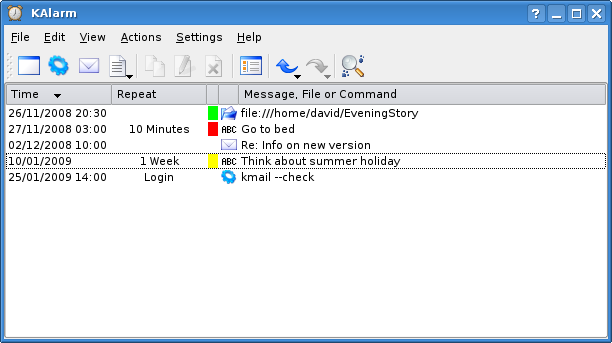
\includegraphics[width=0.7\textwidth]{kalarm.png}
\end{figure}

The program kAlarm allows the user to define some events
(possibly recurrent) and display alarms using pop-up windows
on the screen at times defined by the event. The project should
develop an alternative to this tool, which is platform
independent and open-source.
\chapter{Project Goals}
\section{Goals}
\begin{itemize}
\item Improve the overall life organisation of the user
\item No more missed events
\end{itemize}
\section{Requirements}
\begin{itemize}
\item The application has to be cross platform (Windows, Linux, macOS)
\item The database must not be stored in a binary format
\item The configuration has to be easily transferable to another computer
\item Customisable alerts
\item Classifiable alerts
\item Recurrent alerts
\item Alerts can be scheduled
\item Delay alerts
\item Snooze alerts
%\item Schedule Email Delivery
\end{itemize}
\chapter{System and Context Boundaries}
\lipsum[4-7]
\chapter{System description}
\subsection{User Story \arabic{subsection}: Template}
As an [actor] I want [action] so that [achievement].

\subsubsection{Description}

\subsubsection{Success}

\subsubsection{Failure}
\section{Use Case \arabic{subsection}: Template}

\subsubsection{Scope}

\subsubsection{Primary actor}

\subsubsection{Precondition}

\subsubsection{Postcondition}

\subsubsection{Main success scenario}

\subsubsection{Extension}

%\chapter{Requirements}

\section{User Stories}
As an [actor] I want [action] so that [achievement].
\newcounter{counter}

\subsection{As a User}
\subsubsection{Alerts functionality}
\begin{enumerate}
	\item I want to registrate some alerts so that the software warns me when they occure
	\item I want to be able to chose a different color, font and sound for every alert
	\item I want to edit the existing alerts when needed
	\item I want to delete the existing alerts when needed
	\item I want to postpone an alarm so that i'm notified again later (snooze)
	\item I want to mute an alert so that i'm not notified
	\setcounter{counter}{\value{enumi}}
\end{enumerate}
\subsubsection{Managing alerts}
\begin{enumerate}
	\setcounter{enumi}{\value{counter}}
	\item I want to create categories of alerts, so that I can sort my alerts
	\item I want to edit my categories, in a way my alerts remain categorised
	\item I want to delete categories of alerts, so that my list of categories stay concise
	\item I want to assign color identity to my different categories, some that I can easily find them
	\item I want to personalize the default color, font and sound of my alarms in the software configurations
	\item I want to mute an alert catogory so that i'm not notified by any alert in this category
	\setcounter{counter}{\value{enumi}}
\end{enumerate}
\subsubsection{Persistence}
\begin{enumerate}
	\setcounter{enumi}{\value{counter}}
	\item I want to retrieve the correct state of my alerts after turning my computer down and back on
	\item I want to be alerted at any times, as soon as I'm loged on my computer session
	\setcounter{counter}{\value{enumi}}
\end{enumerate}
\subsubsection{Exportability}
\begin{enumerate}
	\setcounter{enumi}{\value{counter}}
	\item I want to export my alerts so that I can't import then on an other computer with ClockAlarm installed
	\item I want to import an alerts file, so that I can retrieve previously exported alerts
	\item I want to load configuration files, so that I can use predifined color and sound themes
	\setcounter{counter}{\value{enumi}}
\end{enumerate}
\subsubsection{Pivacy}
\begin{enumerate}
	\setcounter{enumi}{\value{counter}}
	\item I want my alerts to remain private, so that nobody except me knows about them
\end{enumerate}

\section{Domain model}
Conceptual model including system behavior and data
\begin{figure}[h]
	\centering
	\caption{Domain model}
	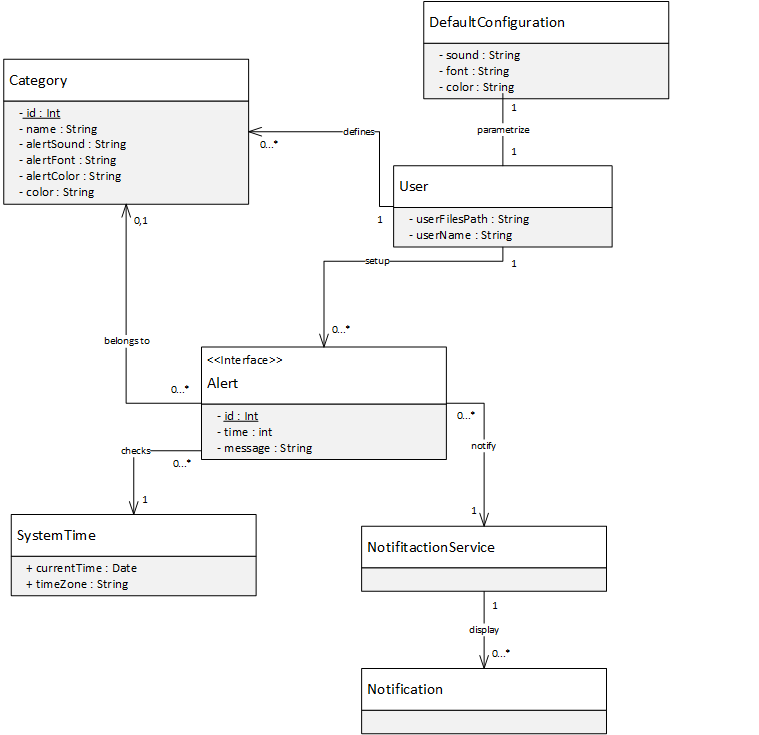
\includegraphics[width=1.0\textwidth]{domain_model.png}
\end{figure}

\section{Use Cases}
\subsection{Program Auto Start}\label{subsec:usecase_auto_start}
TODO
\subsubsection{Scope}

\subsubsection{Primary actor}

\subsubsection{Precondition}

\subsubsection{Postcondition}

\subsubsection{Main success scenario}
\begin{enumerate}
	\item \label{itm:denomination} 
\end{enumerate}
\subsubsection{Extension}
\begin{enumerate}
	\item[\ref{itm:denominationt}.]
	\begin{enumerate}[i]
		\item 
	\end{enumerate}
\end{enumerate}
\subsection{Import Configuration}
Import a ClockAlarm application configuration from an external file.
\subsubsection{Scope}
ClockAlarm application configuration phase.
\subsubsection{Primary actor}
User
\subsubsection{Precondition}
The application has to be started.
\subsubsection{Postcondition}
The application configuration is replaced with the one in the given file.
\subsubsection{Main success scenario}
\begin{enumerate}
	\item The User selects a file to be imported.
	\item\label{itm:ucic_valid_file} The application checks if the file is a valid configuration file.
	\item The application replaces the configuration with the one specified in the file.
	\item The application saves the new configuration.
	\item The application notifies the User that the configuration has been imported successfully.
\end{enumerate}
\subsubsection{Extension}
\begin{enumerate}
	\item[\ref{itm:ucic_valid_file}.] The application detects that the file is invalid.
		\begin{enumerate}[i]
			\item The application notifies the User that the file is invalid.
			\item The User chooses if he wants to select another file.
		\end{enumerate}
\end{enumerate}

\section{Export Configuration}\label{subsec:usecase_export_configuration}
Export a ClockAlarm application configuration to a file.
\subsubsection{Scope}
ClockAlarm application configuration phase.
\subsubsection{Primary actor}
User
\subsubsection{Precondition}
The application has to be started.
\subsubsection{Postcondition}
The application configuration is exported to a file whose path was chosen by the User.
\subsubsection{Main success scenario}
\begin{enumerate}
	\item\label{itm:ucec_save_file} The User is asked where he wants to save the file.
	\item The application exports the configuration to the file.
	\item The application notifies the User that the configuration has been exported successfully.
\end{enumerate}
\subsubsection{Extension}
\begin{enumerate}
	\item[\ref{itm:ucec_save_file}.] The application detects that it has not enough privileges to write to the specified folder.
	\begin{enumerate}[i]
		\item The application notifies the User that it has not enough privileges to write to the specified folder.
		\item The User chooses if he wants to select another folder.
	\end{enumerate}
\end{enumerate}

\subsection{Edit Default Configuration}
Edit the default configuration of the ClockAlarm application.
\subsubsection{Scope}
ClockAlarm application configuration phase.
\subsubsection{Primary actor}
User
\subsubsection{Precondition}
The application has to be started.
\subsubsection{Postcondition}
The application configuration is edited.
\subsubsection{Main success scenario}
\begin{enumerate}
	\item The User edits the configuration
	\item\label{itm:ucedc_second} The application checks if the User entered configuration is valid
	\item The application saves the configuration.
\end{enumerate}
\subsubsection{Extension}
\begin{enumerate}
	\item[\ref{itm:ucedc_second}.] The application detects that the User entered configuration is invalid
		\begin{enumerate}[i]
			\item The application notifies the User that the entered configuration is invalid.
			\item The User chooses if he wants to edit the configuration.
		\end{enumerate}
\end{enumerate}

\section {Launch ClockAlarm manager (no login)}\label{subsec:usecase_launch}
In the case of an application without shared database and user accounts.
\subsubsection{Scope}
A computer running any common operating system (Windows, Mac OS, Linux).
\subsubsection{Primary actor}
User or Administrator
\subsubsection{Precondition}
The computer is on and the user is logged on his computer user session. The ClockAlarm application is correctly installed.
\subsubsection{Postcondition}
ClockAlarm is running and the manager window is open. The user is logged on his personnal ClockAlarm session.
\subsubsection{Main success scenario}
\begin{enumerate}
	\item The user launches the ClockAlarm application.
	\item\label{itm:ucea_start_nl} The application starts and loads configurations and alarms from the user's personal files folder.
	\item\label{itm:ucea_winopen_nl} The manager window opens and displays the main window.
\end{enumerate}
\subsubsection{Extension}
\begin{enumerate}
	\item[\ref{itm:ucea_start_nl}] The application il allready running in background.
	\begin{enumerate}[i]
		\item Goto point~\ref{itm:ucea_winopen_nl}.
	\end{enumerate}
	
	\item[\ref{itm:ucea_start_nl}] Configurations or alerts can not be loaded (e.g.\ first use of the program).
	\begin{enumerate}[i]
		\item The application creates a new default configuration file and an empty alert file.
		\item Goto point~\ref{itm:ucea_start_nl}.
	\end{enumerate}
\end{enumerate}

\section{Launch ClockAlarm manager (with login)}\label{subsec:usecase_launch_log}
In the case of an application with a shared database and user accounts.
\\ \textbf{This solution is unlikely to be kept.}
\\For this reason, not all scenarios, especially those related to the connection with the server, will be treated here.
\subsubsection{Scope}
A computer running any common operating system (Windows, Mac OS, Linux).
\subsubsection{Primary actor}
User or Administrator
\subsubsection{Precondition}
The computer is on and the user is logged on his computer user session. The ClockAlarm application is correctly installed.
\\ The user has a registered user account on the server.
\subsubsection{Postcondition}
ClockAlarm is running and the manager window is open. The user is logged on his personnal ClockAlarm session.
\subsubsection{Main success scenario}
\begin{enumerate}
	\item The user launches the ClockAlarm application.
	\item\label{itm:ucea_start_wl} The application starts. 
	\item\label{itm:ucea_check_wl} The user is asked to enter his credentials and the program tries to check these.
	\item The application is connected to the server.
	\item\label{itm:ucea_load_wl} The application loads configurations and alarms from the server database.
	\item\label{itm:ucea_winopen_wl} The manager window opens and displays the main window.
\end{enumerate}
\subsubsection{Extension}
\begin{enumerate}
	\item[\ref{itm:ucea_start_wl}] The application il allready running in background.
	\begin{enumerate}[i]
		\item Goto point~\ref{itm:ucea_winopen_wl}.
	\end{enumerate}
	
	\item[\ref{itm:ucea_check_wl}] The credentials are incorrect.
	\begin{enumerate}[i]
		\item The connection to the server is denied.
		\item The user is asked to give his credentials again.
		\item Goto point~\ref{itm:ucea_check_wl}.
	\end{enumerate}
	
		\item[\ref{itm:ucea_check_wl}] The user is not registered.
	\begin{enumerate}[i]
		\item The connection to the server is denied.
		\item The user is redirected to a page to an account creation page.
		\item The user creates a new account on the server.
		\item Goto point~\ref{itm:ucea_check_wl}.
	\end{enumerate}
	
	\item[\ref{itm:ucea_load_wl}] Configurations or alerts can not be loaded (e.g.\ first use of the account).
	\begin{enumerate}[i]
		\item The application creates and upload a new default configuration file and an empty alert file.
		\item Goto point~\ref{itm:ucea_start_wl}.
	\end{enumerate}
\end{enumerate}

\section{Setup a new alert: Simple alert}\label{subsec:usecase_add_simple_alert}
A simple alert displays a message to the user at the requested time.
\subsubsection{Scope}
The ClockAlarm manager window.
\subsubsection{Primary actor}
User
\subsubsection{Precondition}
ClockAlarm is running. The configurations and existing alerts are loaded. The user is on the main window.
\subsubsection{Postcondition}
A new simple alert is added to the alert list and is ready to warn the user at the right time.
\subsubsection{Main success scenario}
\begin{enumerate}
	\item The user browse the menu and selects ``File \textgreater~New Alert \textgreater~Simple Alert''. The simple alert creation window is displayed. 
	\item\label{itm:ucaa_enter_sa} The user sets his alert. The message to be displayed as well as the time of display are mandatory. \\The user can, if desired, assign a category to the alert, or set the color, sound and font of the alert.
	\item\label{itm:ucaa_validate_sa} The user validates his alert. The dialog box closes and the manager window is updated.
\end{enumerate}
\subsubsection{Extension}
\begin{enumerate}
	\item[\ref{itm:ucaa_validate_sa}] The user does not complete the category and settings.
	\begin{enumerate}[i]
		\item The default settings are used and the alert does not belong to any category.
	\end{enumerate}
	\item[\ref{itm:ucaa_validate_sa}] The user complete the category, but not the settings.
	\begin{enumerate}[i]
		\item The parameters of the category are used.
	\end{enumerate}
	\item[\ref{itm:ucaa_validate_sa}] One of the parameter is invalid (for example, the time entered is earlier than the current time).
	\begin{enumerate}[i]
		\item The user is asked to check his entries. Back to point~\ref{itm:ucaa_enter_sa}.
	\end{enumerate}
\end{enumerate}

\section{Setup a new alert: Periodic alert}\label{subsec:usecase_add_periodic_alert}
A periodic alert displays a message to the user at the requested periodic time.
\subsubsection{Scope}
The ClockAlarm manager window.
\subsubsection{Primary actor}
User
\subsubsection{Precondition}
ClockAlarm is running. The configurations and existing alerts are loaded. The user is on the main window.
\subsubsection{Postcondition}
A new periodic alert is added to the alert list and is ready to warn the user whenever it occures.
\subsubsection{Main success scenario}
\begin{enumerate}
	\item The user browse the menu and selects ``File \textgreater~New Alert \textgreater~Periodic Alert''. The periodic alert creation window is displayed. 
	\item\label{itm:ucaa_enter_pa} The user sets his alert. The message to be displayed, the time of display as well as the periodicity are mandatory. \\The user can, if desired, assign a category to the alert, or set the color, sound and font of the alert.
	\item\label{itm:ucaa_validate_pa} The user validates his alert. The dialog box closes and the manager window is updated.
\end{enumerate}
\subsubsection{Extension}
\begin{enumerate}
	\item[\ref{itm:ucaa_validate_pa}] The user does not complete the category and settings.
	\begin{enumerate}[i]
		\item The default settings are used and the alert does not belong to any category.
	\end{enumerate}
	\item[\ref{itm:ucaa_validate_pa}] The user complete the category, but not the settings.
	\begin{enumerate}[i]
		\item The parameters of the category are used.
	\end{enumerate}
	\item[\ref{itm:ucaa_validate_pa}] One of the parameter is invalid (for example, the time entered is earlier than the current time).
	\begin{enumerate}[i]
		\item The user is asked to check his entries. Back to point~\ref{itm:ucaa_enter_pa}.
	\end{enumerate}
\end{enumerate}

\section{Setup a new alert: E-mail sender}\label{subsec:usecase_add_email_sender}
An e-mail sender send an e-mail at the requested time.
\subsubsection{Scope}
The ClockAlarm manager window.
\subsubsection{Primary actor}
User
\subsubsection{Precondition}
ClockAlarm is running. The configurations and existing alerts are loaded. The user is on the main window.
\subsubsection{Postcondition}
An e-mail is configured and ready to be sent at the scheduled time.
\subsubsection{Main success scenario}
\begin{enumerate}
    \item The user browse the menu and selects ``File \textgreater~New Alert \textgreater~E-mail Sender''. The e-mail sender creation window is displayed. 
	\item\label{itm:ucaa_enter_es} The user sets his e-mail. He enters the recipient, subject, and body of the message. He also sets the time of sending. \\The user can, if he wants to, enter the path to an attachment.
	\item\label{itm:ucaa_validate_es} The user validates his e-mail. The dialog box closes and the manager window is updated.
\end{enumerate}
\subsubsection{Extension}
\begin{enumerate}
	\item[\ref{itm:ucaa_validate_es}] One of the parameter is invalid (time entered earlier than current time, invalid recipient e-mail address, empty object).
	\begin{enumerate}[i]
		\item The user is asked to check his entries. Back to point~\ref{itm:ucaa_enter_es}.
	\end{enumerate}
\end{enumerate}

\section{Edit an alert: Simple and Periodic alert}\label{subsec:usecase_edit_simple_alert}

\subsubsection{Scope}
The ClockAlarm manager window.
\subsubsection{Primary actor}
User
\subsubsection{Precondition}
ClockAlarm is running. The configurations and existing alerts are loaded. The user is on the main window.
\\A simple(resp. periodic) alert is already set.
\subsubsection{Postcondition}
The selected alert is updated and ready to alert the user at the chosen time.
\subsubsection{Main success scenario}
\begin{enumerate}
	\item The user selects the alert he wishes to modify.
	\item \label{itm:ucae_edit_spa} The user browses the menu and selects ``File \textgreater~Edit Alert''. The simple (resp. periodic) alert edition window is displayed. 
	\item \label{itm:ucae_enter_spa} The current settings are displayed. The user edits his alert. The message to be displayed as well as the time of display (and the periodicity for the periodic alert) are mandatory. \\The user can, if desired, assign or reassign a category, color, sound and font to the alert.
	\item \label{itm:ucae_validate_spa} The user validates his modifications. The edition window closes and the manager window is updated.
\end{enumerate}
\subsubsection{Extension}
\begin{enumerate}
	\item[\ref{itm:ucae_edit_spa}] No alert is selected.
	\begin{enumerate}[i]
		\item Nothing happens.
	\end{enumerate}
	
	\item[\ref{itm:ucae_enter_spa}] The user changes the alert category.
	\begin{enumerate}[i]
		\item The user is asked if he also wants to use the parameters of the category.
	\end{enumerate}
	
	\item[\ref{itm:ucae_validate_spa}] The user does not complete the category and settings.
	\begin{enumerate}[i]
		\item The default settings are used and the alert does not belong to any category.
	\end{enumerate}
	
	\item[\ref{itm:ucae_validate_spa}] The user complete the category, but not the settings.
	\begin{enumerate}[i]
		\item The parameters of the category are used.
	\end{enumerate}
	
	\item[\ref{itm:ucae_validate_spa}] One of the parameter is invalid (for example, the time entered is earlier than the current time).
	\begin{enumerate}[i]
		\item The user is asked to check his entries. Back to point \ref{itm:ucae_enter_spa}.
	\end{enumerate}
\end{enumerate}

\section{Edit an alert: E-mail sender}\label{subsec:usecase_edit_email_sender}

\subsubsection{Scope}
The ClockAlarm manager window.
\subsubsection{Primary actor}
User
\subsubsection{Precondition}
ClockAlarm is running. The configurations and existing alerts are loaded. The user is on the main window.
\\An e-mail sender is already set.
\subsubsection{Postcondition}
The selected e-mail sender is updated and ready to send an e-mail at the scheduled time.
\subsubsection{Main success scenario}
\begin{enumerate}
	\item The user selects the e-mail sender he wishes to modify.
	\item \label The user browses the menu and selects  `` File \textgreater~Edit Alert''. The e-mail sender edition window is displayed. 
	\item \label{itm:ucae_enter_es} The current settings are displayed. The user edits his e-mail. He can edit the recipient, subject, and body of the message. He can also edit the time of sending and the path to an attachment.
	\item \label{itm:ucae_validate_es} The user validates his modifications. The edition window closes and the manager window is updated.
\end{enumerate}
\subsubsection{Extension}
\begin{enumerate}
	\item[\ref{itm:ucae_validate_es}] One of the parameters is invalid (time entered earlier than current time, invalid recipient e-mail address, empty object).
	\begin{enumerate}[i]
		\item The user is asked to check his entries. Back to point \ref{itm:ucae_enter_es}.
	\end{enumerate}
\end{enumerate}

\subsection{Delete an alert: Simple and Periodic alert}

\subsubsection{Scope}
The ClockAlarm manager window.
\subsubsection{Primary actor}
User
\subsubsection{Precondition}
ClockAlarm is running. The configurations and existing alerts are loaded. The user is on the main window.
\\A simple(resp. periodic) alert is already set.
\subsubsection{Postcondition}
The selected alert is deleted won't alert the user in the futur.
\subsubsection{Main success scenario}
\begin{enumerate}
	\item The user selects the alert he wishes to delete.
	\item \label{itm:ucad_delete_spa} The user browses the menu and selects ``File \textgreater~Delete Alert''.
	\item \label{itm:ucad_check_spa} A dialog asks the user to validate his decision.
	\item The alert is deleted. The dialog box closes and the manager window is updated.
\end{enumerate}
\subsubsection{Extension}
\begin{enumerate}
	\item[\ref{itm:ucad_delete_spa}] No alert is selected.
	\begin{enumerate}[i]
		\item Nothing happens.
	\end{enumerate}
	
	\item[\ref{itm:ucad_check_spa}] The user refuses or exits the dialog box.
	\begin{enumerate}[i]
		\item The alert isn't deleted and the dialog box closes.
	\end{enumerate}
\end{enumerate}

\subsection{Delete an alert: E-mail sender}

\subsubsection{Scope}
The ClockAlarm manager window.
\subsubsection{Primary actor}
User
\subsubsection{Precondition}
ClockAlarm is running. The configurations and existing alerts are loaded. The user is on the main window.
\\An e-mail sender is already set.
\subsubsection{Postcondition}
The selected e-mail sender is deleted and won't send any e-mail in the futur.
\subsubsection{Main success scenario}
\begin{enumerate}
	\item The user selects the e-mail sender he wishes to delete.
	\item \label{itm:ucad_delete_es} The user browses the menu and selects ``File \textgreater~Delete Alert''.
	\item \label{itm:ucad_check_es} A dialog asks the user to validate his decision.
	\item The email-sender is deleted. The dialog box closes and the manager window is updated.
\end{enumerate}
\subsubsection{Extension}
\begin{enumerate}
	\item[\ref{itm:ucad_delete_es}] No alert is selected.
	\begin{enumerate}[i]
		\item Nothing happens.
	\end{enumerate}
	
	\item[\ref{itm:ucad_check_es}] The user refuses or exits the dialog box.
	\begin{enumerate}[i]
		\item The email-sender isn't deleted and the dialog box closes.
	\end{enumerate}
\end{enumerate}
\subsection{Setup a new alert category}
Define a category to sort alerts.
\subsubsection{Scope}
The ClockAlarm manager window.
\subsubsection{Primary actor}
User
\subsubsection{Precondition}
ClockAlarm is running. The configurations and existing alerts are loaded. The user is on the main window.
\subsubsection{Postcondition}
A new alert category is created. It defines the parameters of the alerts belonging to it.
\subsubsection{Main success scenario}
\begin{enumerate}
	\item The user browses the menu and selects ``Edit \textgreater~Categories''. The categories manager window is displayed.
	\item The user clicks on the ``New category'' button. The add category dialog is displayed.
	\item\label{itm:ucca_enter_sc}The user defines the new category. The name is mandatory. \\The user can define a font and a color for the alerts and the sound to be used.
	\item\label{itm:ucca_validate_sc} The user validates the category. The category is created
	\item The categories manager window is updated.
	\item The creation window closes.
\end{enumerate}
\subsubsection{Extension}
\begin{enumerate}
	\item[\ref{itm:ucca_validate_sc}] A non-mandatory field is not filled.
	\begin{enumerate}[i]
		\item The default settings are used. 
		\item The category is created.
		\item The categories manager window is updated and the creation window closes.
	\end{enumerate}
	
	\item[\ref{itm:ucca_validate_sc}] One of the parameter is invalid.
	\begin{enumerate}[i]
		\item The user is asked to check his entries. Back to point~\ref{itm:ucca_enter_sc}.
	\end{enumerate}
\end{enumerate}
\section{Edit an alert category}\label{subsec:usecase_edit_category}

\subsubsection{Scope}
The ClockAlarm manager window.
\subsubsection{Primary actor}
User
\subsubsection{Precondition}
ClockAlarm is running. The configurations and existing alerts are loaded. The user is on the main window.
\\A category allready exist.
\subsubsection{Postcondition}
The selected category is updated as wanted. It defines the parameters of the alerts belonging to it.
\\ If alerts are defined by this category, they must be updated too.
\subsubsection{Main success scenario}
\begin{enumerate}
	\item The user browse the menu and selects ``Edit \textgreater~Categories''. The categories manager window is displayed. 
	\item The user selects from the list the category he wishes to modify.
	\item The user clicks on the ``Edit category'' button. The edit category dialog is displayed.
	\item\label{itm:eaac_enter_sc}The user update the selected category. The name is mandatory. \\The user can define or redifine a font and a color for the alerts and the sound to be used.
	\item\label{itm:eaac_validate_sc} The user validates the category. The category is updated, as well as all the alerts it defines.
	\item The categories manager window is updated.
	\item The creation window closes.
\end{enumerate}
\subsubsection{Extension}
\begin{enumerate}
	\item[\ref{itm:eaac_validate_sc}] A non-mandatory field is not filled.
	\begin{enumerate}[i]
		\item The initial setting of this parameter is used. 
		\item The category is updated.
		\item The categories manager window is updated and the dialog box closes.
	\end{enumerate}
	
	\item[\ref{itm:eaac_validate_sc}] One of the parameter is invalid.
	\begin{enumerate}[i]
		\item The user is asked to check his entries. Back to point~\ref{itm:eaac_enter_sc}.
	\end{enumerate}
\end{enumerate}

\section{Delete an alert category}\label{subsec:usecase_delete_category}

\subsubsection{Scope}
The ClockAlarm manager window.
\subsubsection{Primary actor}
User
\subsubsection{Precondition}
ClockAlarm is running. The configurations and existing alerts are loaded. The user is on the main window.
\\A category allready exist.
\subsubsection{Postcondition}
The selected category is deleted.\\The alerts previously defined in this category resume the default configuration.
\subsubsection{Main success scenario}
\begin{enumerate}
	\item The user browse the menu and selects ``Edit \textgreater~Categories''. The categories manager window is displayed. 
	\item The user selects from the list the category he wishes to delete.
	\item The user clicks on the ``Delete category'' button.
	\item\label{itm:uccd_delete_ac} The user is informed that the alerts previously defined by this category will now have the default configuration. The user must accept in order to delete the category.
	\item The category is deleted. The related alerts are updated. The category manager window is updated. 
	\item The dialog box closes.
\end{enumerate}
\subsubsection{Extension}
\begin{enumerate}
	\item[\ref{itm:uccd_delete_ac}] The user refuses or closes the dialog box.
	\begin{enumerate}[i]
		\item The category is not deleted.
		\item The dialog box closes.
	\end{enumerate}
\end{enumerate}

\subsection{Import Alerts}
Load ClockAlarm alerts from an external file.
\subsubsection{Scope}
ClockAlarm application user interface.
\subsubsection{Primary actor}
User
\subsubsection{Precondition}
The application has to be started.
\subsubsection{Postcondition}
New alerts from the given file are added to the alert list.
\subsubsection{Main success scenario}
\begin{enumerate}
	\item The User selects a file to import.
	\item\label{itm:ucia_valid_file} The application checks if the file is a valid alert file.
	\item\label{itm:ucia_import_alerts} The application asks the User which alerts he wants to import.
	\item The application adds the alerts to the User alert list.
	\item The application saves the alert list.
	\item The application notifies the user that the alerts have been imported successfully.
\end{enumerate}
\subsubsection{Extension}
\begin{enumerate}
	\item[\ref{itm:ucia_valid_file}.] The application detects that the file is invalid.
	\begin{enumerate}[i]
		\item The application notifies the user that the file is invalid.
		\item The user chooses if he wants to select another file.
	\end{enumerate}
	\item[\ref{itm:ucia_import_alerts}.] The application detects that the User has chosen no alerts.
	\begin{enumerate}[i]
		\item The application notifies the User that no alerts were chosen to import.
		\item The User chooses if he wants to select alerts to be imported.
	\end{enumerate}
\end{enumerate}

\section{Export Alerts}\label{subsec:usecase_export_alerts}
Export ClockAlarm alerts to a file.
\subsubsection{Scope}
ClockAlarm application user interface.
\subsubsection{Primary actor}
User
\subsubsection{Precondition}
The application has to be started.
\subsubsection{Postcondition}
Alerts are saved to a file whose path was chosen by the User.
\subsubsection{Main success scenario}
\begin{enumerate}
	\item\label{itm:ucea_save_file} The User is asked where he wants to save the file.
	\item\label{itm:ucea_select_alerts} The User selects the alerts he wants to export.
	\item The application exports the alerts to the file.
	\item The application notifies the User that the alerts have been exported successfully.
\end{enumerate}
\subsubsection{Extension}
\begin{enumerate}
	\item[\ref{itm:ucea_save_file}.] The application detects that it has not enough privileges to write to the specified folder.
	\begin{enumerate}[i]
		\item The application notifies the User that it has not enough privileges to write to the specified folder.
		\item The User chooses if he wants to select another folder.
	\end{enumerate}
	\item[\ref{itm:ucea_select_alerts}.] The application detects that the User has chosen no alerts.
	\begin{enumerate}[i]
		\item The application notifies the User that no alerts were chosen to export.
		\item The User chooses if he wants to select alerts to be exported.
	\end{enumerate}
\end{enumerate}

\section{Silent mode ON}\label{subsec:usecase_silent_on}
Mute all the alertes.
\subsubsection{Scope}
The ClockAlarm manager window.
\subsubsection{Primary actor}
User
\subsubsection{Precondition}
ClockAlarm is running. The configurations and existing alerts are loaded. The user is on the main window.
\\Silent mode is disabled.
\subsubsection{Postcondition}
The system is in silent mode. The user will no longer be disturbed by alerts.
\subsubsection{Main success scenario}
\begin{enumerate}
	\item The user browses the menu and selects ``Tool \textgreater~Silent mode''.
	\item In the displayed drop-down menu, the user selects the duration of the mute time.
	\item All alerts are silent for the requested duration.
\end{enumerate}
\subsubsection{Note}
Email alerts can't be muted.

\section{Silent mode OFF}\label{subsec:usecase_silent_off}

\subsubsection{Scope}
The ClockAlarm manager window.
\subsubsection{Primary actor}
User
\subsubsection{Precondition}
ClockAlarm is running. The configurations and existing alerts are loaded. The user is on the main window.
\\Silent mode is enabled.
\subsubsection{Postcondition}
The system is in nomral mode. The user will be alerted on time.
\subsubsection{Main success scenario}
\begin{enumerate}
	\item The user browses the menu and selects ``Tool \textgreater~Silent mode''.
	\item All alarms, except muted ones, are activated again.
\end{enumerate}

\section{Mute a category}\label{subsec:usecase_mute_category}

\subsubsection{Scope}
The ClockAlarm manager window.
\subsubsection{Primary actor}
User
\subsubsection{Precondition}
ClockAlarm is running. The configurations and existing alerts are loaded. The user is on the main window.
\\There is a parameterized and unmuted category.
\subsubsection{Postcondition}
The category is muted. The user will no longer be disturbed by alerts from this category.
\subsubsection{Main success scenario}
\begin{enumerate}
	\item The user browse the menu and selects ``Edit \textgreater~Categories''. The categories manager window is displayed. 
	\item The user selects from the list the category he wishes to mute.
	\item \label{itm:ucmc_mute_mc}The user browses the menu and selects ``Tool \textgreater~Mute''.
	\item In the displayed drop-down menu, the user selects the duration of the mute time.
	\item All alerts from this category are silent for the requested duration.
\end{enumerate}
\subsubsection{Extension}
\begin{enumerate}
	\item[\ref{itm:ucmc_mute_mc}] No category is selected.
	\begin{enumerate}[i]
		\item Option ``Tool \textgreater~Mutes'' is not available.
	\end{enumerate}
\end{enumerate}

\section{Unmute a category}\label{subsec:usecase_unmute_category}

\subsubsection{Scope}
The ClockAlarm manager window.
\subsubsection{Primary actor}
User
\subsubsection{Precondition}
ClockAlarm is running. The configurations and existing alerts are loaded. The user is on the main window.
\\There is a parameterized and muted category.
\subsubsection{Postcondition}
The category is no longer muted. The user will again be alerted on time.
\subsubsection{Main success scenario}
\begin{enumerate}
	\item The user browse the menu and selects ``Edit \textgreater~Categories''. The categories manager window is displayed. 
	\item The user selects from the list the muted category he wishes to unmute.
	\item \label{itm:ucmc_mute_uc}The user browses the menu and selects ``Tool \textgreater~Unmute''.
	\item All alerts from this category are no longer silent and will alert the user on time.
\end{enumerate}
\subsubsection{Extension}
\begin{enumerate}
	\item[\ref{itm:ucmc_mute_uc}] No category is selected.
	\begin{enumerate}[i]
		\item Option ``Tool \textgreater~Unmute is not available.
	\end{enumerate}
\end{enumerate}

\subsection{Snooze Alert}\label{subsec:usecase_snooze_alert}
Snooze the alert on the screen.
\subsubsection{Scope}
ClockAlarm application user interface
\subsubsection{Primary actor}
User
\subsubsection{Precondition}
The application has to be started. A default configuration file exists.
\subsubsection{Postcondition}
The alert is snoozed for a certain amount of time.
\subsubsection{Main success scenario}
\begin{enumerate}
    \item The User snoozes the alert.
    \item\label{itm:ucsa_no_config_found} The application changes the alert 
        time of the specific alert and adds an amount of time defined by the
        configuration.
\end{enumerate}
\subsubsection{Extension}
\begin{enumerate}
	\item[\ref{itm:ucsa_no_config_found}.] The application can't find the 
        configuration.
		\begin{enumerate}[i]
			\item The application notifies the User that the configuration
                has not been found.
			\item The application uses the time defined in the default 
                configuration.
		\end{enumerate}
\end{enumerate}


\section{Priorities and planning}\label{sec:prio_and_planning}
Description of the various stages of development of the ClockAlarm product. The versions correspond to the fixed milestones. For each element, a priority is associated.

Priorities: \gls{mh}, \gls{p1}, \gls{p2}, \gls{nth}

\setlength\tabcolsep{2pt}
\begin{longtable}{| c | p{5cm} | c | c | p{5cm} |}
	\caption{Priorities Table}\\
	\hline
	\rowcolor{beaublue}\textbf{Vers.} & \textbf{To Implement} & \textbf{Prio} & \textbf{Status} & \textbf{Description} \\
	\boldhr
	\endfirsthead
	\multicolumn{5}{c}{\tablename\ \thetable\ -- \textit{Continued from previous page}} \\
	\hline
	\rowcolor{beaublue}\textbf{Vers.} & \textbf{To Implement} & \textbf{Prio} & \textbf{Status} & \textbf{Description} \\
	\boldhr
	\endhead
	
	\hline \multicolumn{5}{r}{\textit{Continued on next page}} \\
	\endfoot
	\hline
	\endlastfoot
	
	\rowcolor{aliceblue}0.2.0 & Time System and Notifications & \gls{mh} & Done & The program is able to display a hard coded alert, based on the operating system time \\ \hline
	\rowcolor{aliceblue}0.2.1 & \fullref{subsec:usecase_launch} & \gls{p2} & Done & The scheduled alert is visible in a GUI before it occures \\ \boldhr
	0.3.0 & Persistence \& Start at Runtime & & Partially done & At run-time, the program is launched and starts popping alerts. The previously saved alerts are retrieved \\ \hline
	& \fullref{subsec:usecase_auto_start} & NTH & Not done\footnote{\label{ftn:autostart}See~\fullref{sec:unimplreq}, \textit{Auto start}} & \\ \boldhr
	\rowcolor{aliceblue}1.0.0 & Add/Delete/Edit Alerts & & Partially done &  \\ \hline
	\rowcolor{aliceblue}& \fullref{subsec:usecase_add_simple_alert} & MH & Done &  \\ \hline
	\rowcolor{aliceblue}& \fullref{subsec:usecase_delete_simple_alert} & MH & Done &  \\ \hline
	\rowcolor{aliceblue}& \fullref{subsec:usecase_edit_simple_alert} & MH & Done &  \\ \hline
	\rowcolor{aliceblue}& \fullref{subsec:usecase_add_periodic_alert} & \gls{p1} & Done &  \\ \hline
	\rowcolor{aliceblue}& \fullref{subsec:usecase_add_email_sender} & \gls{nth} & Not done\footnote{\label{ftn:emailreq}See~\fullref{sec:unimplreq}, \textit{Email alert}} &  \\ \hline
	\rowcolor{aliceblue}& \fullref{subsec:usecase_delete_email_sender} & NTH & Not done\footref{ftn:emailreq} &  \\ \hline
	\rowcolor{aliceblue}1.0.1 & \fullref{subsec:usecase_edit_email_sender} & NTH & Not done\footref{ftn:emailreq} &  \\ \boldhr
	1.1.0 & Default Configurations \& Alerts Management &  & Done & The user can change the default settings. The user can import and export lists of alerts\\ \hline
	& \fullref{subsec:usecase_edit_default_configuration} & MH & Done & \\ \hline
	& \fullref{subsec:usecase_import_alerts} & P1 & Done & \\ \hline
	1.1.1 & \fullref{subsec:usecase_export_alerts} & P1 & Done &\\ \boldhr
	\rowcolor{aliceblue}1.2.0 & Categories & & Not done\footnote{\label{ftn:categories}See~\fullref{sec:unimplreq}, \textit{Alert categories}} & The user can create, edit and delete categories \\ \hline
	\rowcolor{aliceblue}& \fullref{subsec:usecase_add_category} & MH & Not done\footref{ftn:categories} & \\ \hline
	\rowcolor{aliceblue}& \fullref{subsec:usecase_delete_category} & MH & Not done\footref{ftn:categories} & \\ \hline
	\rowcolor{aliceblue}1.2.1 & \fullref{subsec:usecase_edit_category} & P2 & Not done\footref{ftn:categories} & \\ \boldhr
	1.3.0 & Import/Export Configuration File &  & Done & \\ \hline
	& \fullref{subsec:usecase_import_configuration} & MH & Done & \\ \hline
	& \fullref{subsec:usecase_export_configuration} & MH & Done & \\ \boldhr
	\rowcolor{aliceblue}1.4.0 & Disable Notifications &  & Partially done & The user is able to prevent certain alerts from taking place.\\ \hline
	\rowcolor{aliceblue}& \fullref{subsec:usecase_silent_on} & MH & Done & \\ \hline
	\rowcolor{aliceblue}& \fullref{subsec:usecase_silent_off} & MH & Done & \\ \hline
	\rowcolor{aliceblue}& \fullref{subsec:usecase_mute_category} & P2 & Not done\footref{ftn:categories} & \\ \hline
	\rowcolor{aliceblue}1.4.1 & \fullref{subsec:usecase_unmute_category} & P2 & Not done\footref{ftn:categories} & \\ \boldhr
	1.5.0 & Snooze Alert & NTH & Not done\footnote{\label{ftn:snooze}See~\fullref{sec:unimplreq}, \textit{Snooze alert}} & The user can ask an alert to ring again in the future. \\ \hline
	& \fullref{subsec:usecase_snooze_alert} & NTH & Not done\footref{ftn:snooze} & \\ \boldhr
	\rowcolor{aliceblue}1.6.0 & Handback the Code & MH & Waiting & The deadline is 2 June 2017 \\ \hline
\end{longtable}


\section{Technical Requirements}
\label{sec:tech_req}

The priorities are the same as in~\ref{sec:prio_and_planning}, i.e., Must Have
(MH), First Priority (P1), Second Priority (P2), Nice To Have (NTH).

\tabulinesep = 1mm
\begin{longtabu}{lccX}
\caption{Technical Requirements Table}
\label{tabu:tech_req}\\

    %\toprule
    \taburowcolors~{beaublue..beaublue}
    \textbf{ID}  & \textbf{Status} & \textbf{Prio}  & \textbf{Description}\\
    \taburowcolors~{white..white}
    %\midrule
    \endfirsthead\\

    %\toprule
    \taburowcolors~{beaublue..beaublue}
    \textbf{ID}  & \textbf{Status} & \textbf{Prio}  & \textbf{Description}\\
    \taburowcolors~{white..white}
    %\midrule
    \endhead\\
    
    \taburowcolors~{white..white}
    \multicolumn{4}{r}{\textit{Continued on next page}}\\
    \endfoot
    %\bottomrule
    \endlastfoot


    \taburowcolors~{aliceblue..white}
    T.1 & Waiting  & MH & The application shall be written using the python
                          programming language version 3 or greater.\\%\midrule
    T.2 & Waiting  & MH & The application shall run on Windows, Linux and
                          macOS.\\%\midrule
    T.3 & Done  & MH & The database shall be stored in a non binary format.
                          \\%\midrule
    T.4 & Waiting  & MH & The application shall still be running after a system
    reboot.\\%\midrule
    T.5 & Waiting  & MH & The configuration file shall be OS independent.\\
    \taburowcolors~{white..white}

\end{longtabu}


\section{Quality Requirements}

The priorities are again the same as in~\ref{sec:prio_and_planning}
and~\ref{sec:tech_req}.

\begin{longtabu}{cccX}
\caption{Quality Requirements Table}
\label{tabu:qual_req}\\
    
    \toprule
    \taburowcolors~{beaublue..beaublue}
    \textbf{ID}  & \textbf{Status} & \textbf{Prio}  & \textbf{Description}\\
    \taburowcolors~{white..white}
    \toprule
    \endfirsthead\\

    \multicolumn{4}{c}{\tablename\ \thetable\ --- \textit{Continued from
    previous page}} \\

    \toprule
    \taburowcolors~{beaublue..beaublue}
    \textbf{ID}  & \textbf{Status} & \textbf{Prio}  & \textbf{Description}\\
    \taburowcolors~{white..white}
    \toprule
    \endhead\\
    
    \taburowcolors~{white..white}
    \multicolumn{4}{r}{\textit{Continued on next page}}\\
    \endfoot
    \bottomrule
    \endlastfoot

    \taburowcolors~{aliceblue..white}
    Q.1 & Waiting  & MH & The application shall display an alert on the screen
    within a second at the specified date and time of the alert.\\\midrule
    Q.2 & Waiting  & MH & The user shall be able to snooze an alert appearing
    on the screen.\\\midrule
    Q.3 & Waiting  & P1 & The user interface shall contain buttons and be user
    friendly.\\

    \taburowcolors~{white..white}

\end{longtabu}


\chapter{Development decisions}

The structure of the development process of this project is based on the book
`Requirements Engineering Fundamentals`\cite{pohl2011requirements}.

\subsection{Word Processor}
In order to write this document, we had to choose between several word processors. We required that the file could be used with a version control system so that the documentation and code could live in the same place. Also, we didn't want to loose time if there was a need to change the layout. After discussion, we came up with the following list:
\begin{enumerate}
\item \Gls{microsoft_word}
\item \Gls{google_docs}
\item \Gls{libre_office}
\item \Gls{scribus}
\item \Gls{tex}
\end{enumerate}
The main problem with number 1 and 3 is that the output of these programs are binary files. A built in versioning functionality exits in \gls{microsoft_word} but it adds another version control layer to the workflow. The .docx and .odt file types are in fact ZIP archives containing XML documents which can be uncompressed. They could be stored in the uncompressed state to be compatible with the chosen version control system \cite{zipdocextension}. Or they could be converted into another format. Clearly this is not convenient. Therefore we decided that they were not compatible with our first requirement stated above.\\
Using a Google Doc means that the document will be stored on Google's servers and not within the folder containing the source code. I thus also violates our first requirement.\\
\Gls{scribus} is a free alternative to \gls{indesign} and doesn't produce binary files. It allows a fine-grained control of the layout, frames and styles \cite{ibm2013open}.\\
Finally there is \gls{tex}, a typesetting system created by Knuth. It provides a low-level language that is not directly used when writing documents. Instead there exist higher level formats such as \gls{latex} or Plain \TeX (much more lower level than \gls{latex}) which provide a large set of macros \cite{levels2017}.\\
Our supervisor strongly recommended us the use of \gls{latex}, that is why we ended up using it.
\chapter{Version Control}\label{ch:version}

\tabulinesep = 1mm
\begin{longtabu}{lccX}
\caption{Version Control Table}
\label{tabu:tech_req}\\
    %\toprule
    \taburowcolors~{beaublue..beaublue}
    \textbf{Version}  & \textbf{Date} & \textbf{Description}  & \textbf{Author}\\
    \taburowcolors~{white..white}
    %\midrule
    \endfirsthead\\
    %\toprule
    \taburowcolors~{beaublue..beaublue}
    \textbf{Version}  & \textbf{Date} & \textbf{Description}  & \textbf{Author}\\
    \taburowcolors~{white..white}
    %\midrule
    \endhead\\
    
    \taburowcolors~{white..white}
    \textbf{Version}  & \textbf{Date} & \textbf{Description}  & \textbf{Author}\\
    \endfoot
    %\bottomrule
    \endlastfoot
    \taburowcolors~{aliceblue..white}
    X0.1 & 26.02.2017 & Initialization of the requierments document  & Samuel Gauthier\\%\midrule
    X0.2 & 13.03.2017  & Update of the requierments documentation & Loïc Charrière\\%\midrule
    X1.0 & 28.05.2017  & Document ready for review & Samuel Gauthier\\%\midrule
    V1.0 & 29.05.2017  & Document ready for handout & Loïc Charrière\\
    V1.4 & 10.06.2017  & Document revision & Samuel Gauthier\\
    \taburowcolors~{white..white}
\end{longtabu}

\subsection{Python}
\section{Unit Testing}
\section{Code Coverage}

There is at the moment only one maintained mature tool for measuring the code
coverage in Python: Coverage.py.\footnote{Nose provides code coverage but it is
deprecated and being replaced by nose2, still under development.} ``It monitors
your program, noting which parts of the code have been executed, then analyzes
the source to identify code that could have been executed but was
not.''\cite{coveragePY} It also provides clean and readable annotated html
reports.

\section{Continuous Integration}

We chose to use \gls{travis}
\footnote{\url{https://travis-ci.org/BFH-BTI7301-project1/ClockAlarm}}, the
\gls{continuous_integration} service. Every time a commit is made, the entire
project is build and the tests are run. Then the report is sent to
Coveralls\footnote{\url{https://coveralls.io/github/BFH-BTI7301-project1/%
ClockAlarm?branch=master}}. This approach allows us to have a better development
workflow.

\section{Documentation}
\label{sec:documentation}

For documenting our project we use Sphinx
\footnote{\url{http://www.sphinx-doc.org}} combined with Read
The Docs\footnote{\url{https://readthedocs.org}} to host the
documentation. Read The Docs builds the documentation every time there is a new
commit (A git hook has to be set up beforehand for it to work).

We choose Sphinx because it is the most popular tool used in the python
community and it is officially recommended (The official Python documentation is
created using Sphinx).

During development we realised thanks to Sphinx that our project had cycles. See
Section~\ref{sec:cycles} for additional details.

After retrospection, this document could have been written using Sphinx. It has
the same capabilities than \LaTeX{} and can generate the document in multiple
formats: pdf, html, etc..

\section{System Notifications}

We first tried to use the OS specific system notification API.\@With this
solution we didn't have to care were the notifications would appear on the
screen. They would always be at the correct position on every platform. There is
however one drawback: the notifications cannot be fully customized. Only the
icon can be changed but the typeface and the sound cannot. This is why we choose
to develop our own notification system, \texttt{Notification.py}, where
notifications can be fully customized.

\section{GUI}

As our application has to run on multiple platforms, the GUI framework should
also support multiple platforms. The framework should also support Python 3. The
Python wiki lists over 35 frameworks, many of those target \gls{qt}. We have chosen
only three that were recommended by the
\citetitle{schlusser2016hitchhikers}~\cite{schlusser2016hitchhikers}:

\begin{enumerate}
    \item PySide
    \item PyQt
    \item Tk
\end{enumerate}

PySide, as PyQt, provides a binding to the \gls{qt} framework. The main difference
between the two is the license: PySide uses the \acrfull{lgpl} whereas PyQt uses
the \acrfull{gpl}. Which means that source code licensed under the
\acrshort{gpl} must be opensource. On the other hand the
\acrshort{lgpl} is more suited for closed source projects. In addition PyQt
supports Python 3. Tk provides bindings to the Tk framework and is licensed
under a \acrfull{bsd} license.

We chose the PyQt framework out of personal preference. All three frameworks
are equally well suited for a project like this one.




\section{Database}

We planned to have three alert types:

\begin{enumerate}
    \item Simple non recurring text alerts
    \item Recurring simple alerts
    \item Alerts that send emails
\end{enumerate}

All three types are independent of each other, that is, there is no logical link
between them. The only ``link'' that they have in common is that they are
extending the abstract class \texttt{Alert}. Therefore we don't need a
relational database, only a very lightweight one.

The requirement for the file storing the database is that it should be humanly
readable, i.e., it should be in a non binary format. We came up with four
possibilities for the file format:

\begin{itemize}
    \item XML
    \item JSON
    \item YAML
    \item Plaintext
\end{itemize}

BaseX\footnote{For python it is the BaseXCLient:
\url{http://basex.org}} handles both JSON and XML databases. Another
alternative is TinyDB
\footnote{\url{http://tinydb.readthedocs.io}}, it
handles only databases in the JSON format. PyXAML
\footnote{\url{http://pyyaml.org}} handles databases stored in the
YAML
format. And for a plaintext database, i.e., a simple text file, everything has
to be handled with the Python \texttt{open(\ldots)} and \texttt{write(\ldots)}
commands.

We choose to use TinyDB and the JSON file format because our supervisor
encouraged us to do so and because the syntax is very simple and follows the
Pythonic way.

\section{Sound}\label{sec:sound}

We had an issue on macOS and linux when using PyQt's \texttt{QSound} class.
\texttt{QSound} uses the default OS specific sound library to play the sound
(NSSound for macOS and \gls{nasl} for X11 used on linux). The \texttt{wav} file
only played on Windows but not on macOS nor linux.

An easier and much cleaner alternative was found using pygame's \texttt{mixer}.


\section{Cycles}
\label{sec:cycles}

As already mentioned in Section~\ref{sec:documentation} Sphinx made us aware of
cycles in our code:

\begin{enumerate}

    \item \texttt{SimpleAlert}~$\rightlcurvearrow$~\texttt{main}
        $\rightlcurvearrow$~\texttt{AlertCollction}~$\rightlcurvearrow$
        \texttt{SimpleAlert}

        The \texttt{SimpleAlert} class was directly accessing
        the \texttt{AlertCollection} inside of \texttt{main} to
        delete \texttt{SimpleAlert}s or update periodic \texttt{SimpleAlert}s.
        The code doing the \texttt{SimpleAlert} update and delete has been moved
        to the \texttt{check\_timers(self, trig\_time)} method inside of
        \texttt{AlertCollection}.

    \item \texttt{AlertCollection}~$\rightlcurvearrow$~\texttt{main}
        $\rightlcurvearrow$~\texttt{AlertCollection}

        The \texttt{display(self)} method in \texttt{AlertCollection} triggered
        the actualization method of the \texttt{UI.AlertListWidget} from the
        \texttt{App} in \texttt{main}.

\end{enumerate}



\section{Metaclass}

A metaclass issue was discovered when we tried to apply the new python 3 style
for abstract classes. In our case, the \texttt{Alert} class is an abstract class
that extends \texttt{QObject}. As \texttt{QObject} has its metaclass, pyhton
could not resolve which metaclass \texttt{Alert} should inherit. Therefore a
special metaclass \texttt{AlertMeta} had to be created. It inherits
\texttt{QObject}'s metaclass and is abstract. The \texttt{Alert} class then
has the metaclass \texttt{AlertMeta} and extends
\texttt{QObject}.~\cite{sim2017meta,maries2015meta}

The difference is shown in Listings~\ref{metapy2} and~\ref{metapy3}.

\lstdefinestyle{custompy}{
  belowcaptionskip=1\baselineskip,
  breaklines=true,
  frame=l,
  xleftmargin=\parindent,
  language=Python,
  showstringspaces=false,
  basicstyle=\footnotesize\ttfamily,
  keywordstyle=\bfseries\color{green!40!black},
  commentstyle=\itshape\color{purple!40!black},
  identifierstyle=\color{blue},
  stringstyle=\color{orange},
}
\lstset{style=custompy,caption={Abstract class, Python 2.7},label=metapy2}
\begin{lstlisting}
...
class Alert(PyQt5.QtCore.QObject):
    __metaclass__ = abc.ABCMeta
    ...
\end{lstlisting}

\lstset{style=custompy,caption={Abstract class, Python 3.6},label=metapy3}
\begin{lstlisting}
...
class AlertMeta(type(PyQt5.QtCore.QObject), abc.ABC):
    pass

class Alert(pyqt.QObject, metaclass=AlertMeta):
    ...
\end{lstlisting}

\section{Unimplemented Requirements}\label{sec:unimplreq}

Due to the time constraint the following requirements could not be fulfilled:

\begin{itemize}

    \item \textbf{Alert categories:}
        \fullref{subsec:usecase_add_category},
        \fullref{subsec:usecase_delete_category},
        \fullref{subsec:usecase_edit_category},
        \fullref{subsec:usecase_mute_category},
        \fullref{subsec:usecase_unmute_category}, Q.2.2 The main user interface
        shall contain buttons to create, edit, delete categories, Q.2.6 The user
        shall be able to sort the alerts by category, by due date and
        alphabetically.

    \item \textbf{Email alert:}
        \fullref{subsec:usecase_add_email_sender},
        \fullref{subsec:usecase_delete_email_sender},
        \fullref{subsec:usecase_edit_email_sender}. These requirements do not
        really make sense because they allready exist in Outlook\footnote{\url{
                https://support.office.com/en-us/article/Delay-or-schedule%
                -sending-email-messages-026af69f-c287-490a-a72f-6c65793744ba}}
                and Thunderbird\footnote{\url{https://addons.mozilla.org/en-US/%
                thunderbird/addon/send-later-3/?src=search}}

     \item \textbf{Snooze alert:}
         \fullref{subsec:usecase_snooze_alert}

     \item \textbf{Auto start:}
         \fullref{subsec:usecase_auto_start}, T.4 The application shall still be
         running after a system reboot.


\end{itemize}

\subsubsection{SimpleAlert class}

The existence of a \texttt{SimpleAlert} and \texttt{Alert} class can seem to be
unoptimized at first glance. The two classes could have been merged together.
But in our initial development decisions, we planned to add another class
extending \texttt{Alert}, namely \texttt{EmailAlert}. We decided to leave the
design like it is now, so that it is easier to create a custom alert class in
the future.


\chapter{Minutes}
\section{Meeting~\arabic{section}: March 1, 2017}
\subsection*{Present at meeting}
Samuel Gauthier, Loïc Charrière, Claude Fuhrer
\subsection*{Agenda}
\begin{itemize}
	\item Present  the Use Cases  and User stories
	\item Discussion about the usage of Python
\end{itemize}
\subsection*{Notes}
	\subsubsection{Use Cases and User stories}
	\begin{itemize}
        	\item Vision\&Goals: The vision and goals of the project have to be enhanced and not taken ``as is''.
		\item If a choice is made during the project, we should write down why it has been made this way. Everything that hasn't been documented is considered not been done.
		\item If we go for a specific product (such as DBMS, module, etc.) we should at least try out other alternatives (2--3) and explain why we made the choice of using this specific product.
		\item Split the user story ``reate/delete categories'' in two.
		\item Sort the uses cases by topic.
		\item Alarms could be snoozed. (for example, if the user is at a meeting snooze all alarms so that they don't disturb the meeting) 
		\item Alarms should be user specific, i.e., they should belong to the user connected on the computer and not be shared across all the users of the machine.
		\item Book recommendation (chapter about use cases) -> Applying UML and Patterns (Larman).
	\end{itemize}
	\subsubsection{Usage of Python}
	\begin{itemize}
		\item Strongly discouraged to share python code via e-mail (General life advice)
		\item Code coverage 70--80\% is ok, 30\% is not
        \end{itemize}
\subsection*{Tasks}
	\begin{itemize}
		\item Improve vision\&goals
		\item Create use cases / user stories / actors correctly
		\item Read Python doc
	\end{itemize}
\subsection*{Next Meeting}
\st{TBD} (edit)
March 17, 2017

\section{Meeting~\arabic{section}: March 17, 2017}
\subsection*{Present at meeting}
Samuel Gauthier, Loïc Charrière, Claude Fuhrer
\subsection*{Agenda}
\begin{itemize}
    \item System and Context Boundaries
    \item System diagrams
    \item System description
\end{itemize}
\subsection*{Notes}
    The Project Goals should not be written down as a list. We need to create
    full sentences in order to help the reader's comprehension.\\
    \textbf{Question:} ``Should this document contain snippets of code?''\\
    \textbf{Answer:} It depends on the target audience. But here we should
    only show snippets of pseudo code for complicated parts of our code.
    \subsubsection{System and Context Boundaries}
    \begin{itemize}
        \item Some of the Stakeholders will not influence our project. They
            are only there so that our documentation is complete.
    \end{itemize}
    \subsubsection*{System diagrams}
    \begin{itemize}
        \item Good domain model.
        \item The domain model should contain types only if they
            are very specific and part of the DM\@.
        \item It is not useful to specify interfaces and abstract classes.
    \end{itemize}
    \subsubsection*{System description}
    \begin{itemize}
        \item We need to link the User Stories and Use Cases.
    \end{itemize}
    \subsection*{Other}
    \textbf{Question:} ``How should our workflow be? Should we write the
    documentation and the code at the same time?''\\
    \textbf{Answer:} We shouldn't waste too much time on writing documentation.
    Basically we should use the Scrum method. All the Use Cases (or the most
    important ones) have to be written down. Then we can decide what has to
    be included in each sprints. For each sprint we must have a working version
    of our application. Start with a small version having the alerts date
    hard coded in the code, with no GUI.\@ Then add a new feature with each
    sprints.
\subsection*{Tasks}
    \begin{itemize}
        \item Rewrite the Project Goals
        \item Prepare sprints
    \end{itemize}
\subsection*{Next Meeting}
TBD



%\clearpage

\printglossaries

\printbibliography[
heading=bibintoc,
title={Bibliography}
]

\end{document} 